\chapter{元组}
\label{元组}

\section{元组是不可变的}

\index{元组}
\index{类型!元组}
\index{序列}

元组是一组序列的值。元组中的值可以是任何数据类型,使用整数作为下标,在这个方面元组很想列表。但是一个主要的区别是元组是不可改变的。

\index{可改变的}
\index{不可改变的}

从语法构成上来看,元组是用逗号隔开的值的序列:

\beforeverb
\begin{verbatim}
>>> t = 'a', 'b', 'c', 'd', 'e'
\end{verbatim}
\afterverb
%
通常用括号包含元组,虽然这不是必要的:

\index{括号!元组位于}

\beforeverb
\begin{verbatim}
>>> t = ('a', 'b', 'c', 'd', 'e')
\end{verbatim}
\afterverb
%
要创建只含一个元素的元组,你需要包含最后的逗号:

\index{单一}
\index{元组!单一}

\beforeverb
\begin{verbatim}
>>> t1 = 'a',
>>> type(t1)
<type 'tuple'>
\end{verbatim}
\afterverb
%
在括号中的值不是元组:

\beforeverb
\begin{verbatim}
>>> t2 = ('a')
>>> type(t2)
<type 'str'>
\end{verbatim}
\afterverb
%
创建元组的另一个方式是使用内减函数{\tt tuple}。当没有参数时,函数创建一个空的元组:

\index{tuple函数}
\index{函数!tuple}

\beforeverb
\begin{verbatim}
>>> t = tuple()
>>> print t
()
\end{verbatim}
\afterverb
%
如果参数是一个序列(字符串、列表或元组),返回结果是使用序列中的元素构成的元组:

\beforeverb
\begin{verbatim}
>>> t = tuple('lupins')
>>> print t
('l', 'u', 'p', 'i', 'n', 's')
\end{verbatim}
\afterverb
%
由于{\tt tuple}是一个内建函数的名字,你应该避免使用它作为变量名。

大多数的列表运算符适用于元组。括号运算符可以索引一个元素:

\index{括号运算符}
\index{运算符!括号}

\beforeverb
\begin{verbatim}
>>> t = ('a', 'b', 'c', 'd', 'e')
>>> print t[0]
'a'
\end{verbatim}
\afterverb
%
切片运算符选择一个范围内的元素。

\index{切片运算符}
\index{运算符!切片}
\index{元组!切片}
\index{切片!元组}

\beforeverb
\begin{verbatim}
>>> print t[1:3]
('b', 'c')
\end{verbatim}
\afterverb
%
但是如果你试图修改元组中的元素,你会得到错误:

\index{异常!类型错误}
\index{类型错误}
\index{项目赋值}
\index{赋值!项目}

\beforeverb
\begin{verbatim}
>>> t[0] = 'A'
TypeError: object doesn't support item assignment
\end{verbatim}
\afterverb
%
你不能修改一个元组的元素,但是你可以使用另一个元组代替原来的元组:

\beforeverb
\begin{verbatim}
>>> t = ('A',) + t[1:]
>>> print t
('A', 'b', 'c', 'd', 'e')
\end{verbatim}
\afterverb
%

\section{元组赋值}
\label{元组赋值}

\index{元组!赋值}
\index{赋值!元组}
\index{交换模式}
\index{模式!交换}

我们经常会用到两个变量间的值的交换。对于传统的赋值,你需要使用一个临时变量。例如,要交换{\tt a}和{\tt b}:

\beforeverb
\begin{verbatim}
>>> temp = a
>>> a = b
>>> b = temp
\end{verbatim}
\afterverb
%
这个方法显得笨拙,{\bf 元组赋值}就优雅许多:

\beforeverb
\begin{verbatim}
>>> a, b = b, a
\end{verbatim}
\afterverb
%
左侧是变量组成的元组,右侧是表达式组成的元组。每个值被赋值给对应的变量。右侧所有的表达式被计算后再赋值。

左侧的变量个数必须等于右侧值的个数:

\index{异常!值错误}
\index{值错误}

\beforeverb
\begin{verbatim}
>>> a, b = 1, 2, 3
ValueError: too many values to unpack
\end{verbatim}
\afterverb
%
更一般的,右侧可以是任何序列(字符串、列表或元组)。例如,要分离一个email地址的用户名和域,你可以这么写:

\index{split方法}
\index{方法!split}
\index{email地址}

\beforeverb
\begin{verbatim}
>>> addr = 'monty@python.org'
>>> uname, domain = addr.split('@')
\end{verbatim}
\afterverb
%
{\tt split}的返回值是两个元素的列表。第一个元素被赋值给{\tt uname},第二个被赋值给{\tt domain}。

\beforeverb
\begin{verbatim}
>>> print uname
monty
>>> print domain
python.org
\end{verbatim}
\afterverb
%

\section{元组作为返回值}

\index{元组}
\index{值!元组}
\index{返回值!元组}
\index{函数,元组作为返回值}

严格地说,一个函数只能返回一个值,但是如果这个值是一个元组,等效于返回多个值。例如,如果你要计算两个整数的除法并得到商和余数,分别计算{\tt x/y}和{\tt x\%y}的效率太低,一个好的方法是同时计算这两个值。

\index{divmod}

内建函数{\tt divmod}读取两个参数,返回有两个值的元组,分别是商和余数。你可以将结果保存在一个元组中:

\beforeverb
\begin{verbatim}
>>> t = divmod(7, 3)
>>> print t
(2, 1)
\end{verbatim}
\afterverb
%
或者使用元组赋值将元素分开保存:

\index{元组赋值}
\index{赋值!元组}

\beforeverb
\begin{verbatim}
>>> quot, rem = divmod(7, 3)
>>> print quot
2
>>> print rem
1
\end{verbatim}
\afterverb
%
下面给出一个返回元组的函数的例子:

\beforeverb
\begin{verbatim}
def min_max(t):
    return min(t), max(t)
\end{verbatim}
\afterverb
%
{\tt max}和{\tt min}是内建函数,分别查找序列中最大和最小的元素, \verb"min_max"计算两者并返回包含两个值的元组。

\index{max函数}
\index{函数!max}
\index{min函数}
\index{函数!min}


\section{变长参数元组}

\index{变长参数元组}
\index{参数!变长元组}
\index{聚集}
\index{参数!聚集}
\index{参数!聚集}

函数可以读取一个变长的参数。一个以{\tt *}开头的参数将参数{\bf 聚集}为一个元组。例如,{\tt printall}可以接收任意个数的参数,并打印它们:

\beforeverb
\begin{verbatim}
def printall(*args):
    print args
\end{verbatim}
\afterverb
%
聚集的参数可以取任何你喜欢的名字,但是习惯上使用{\tt args}。下面给出函数是如何工作的:

\beforeverb
\begin{verbatim}
>>> printall(1, 2.0, '3')
(1, 2.0, '3')
\end{verbatim}
\afterverb
%
和聚集相对应的是{\bf 散布}。如果你有一个值的序列要作为多个参数传给一个函数,你可以使用{\tt *}运算符。例如,{\tt divmod}需要两个参数,而不是一个元组:

\index{散布}
\index{参数散布}

\index{类型错误}
\index{异常!类型错误}

\beforeverb
\begin{verbatim}
>>> t = (7, 3)
>>> divmod(t)
TypeError: divmod expected 2 arguments, got 1
\end{verbatim}
\afterverb
%
但是如果你散布元组,它将工作正常:

\beforeverb
\begin{verbatim}
>>> divmod(*t)
(2, 1)
\end{verbatim}
\afterverb
%
\begin{ex}
许多内建函数使用变长参数元组。例如,{\tt max}和{\tt min}可以读取任意个数的参数:

\index{max函数}
\index{函数!max}
\index{min函数}
\index{函数!min}

\beforeverb
\begin{verbatim}
>>> max(1,2,3)
3
\end{verbatim}
\afterverb
%
但是{\tt sum}函数不是这样。

\index{sum函数}
\index{函数!sum}

\beforeverb
\begin{verbatim}
>>> sum(1,2,3)
TypeError: sum expected at most 2 arguments, got 3
\end{verbatim}
\afterverb
%
编写函数{\tt sumall},可以接收任意多个参数,并返回它们的和。

\end{ex}


\section{列表和元组}

\index{zip函数}
\index{函数!zip}

{\tt zip}是一个内建函数,参数为两个或两个以上的序列,并将它们“拉链”成一个元组的列表,每个元组包含每个序列中的一个元素\footnote{在Python 3.0中,{\tt zip}返回一个元组的迭代器,但是对于大多数情况,迭代器表现的像一个列表。}。

\index{Python 3.0}

下面是一个字符串和一个列表的拉链的例子:

\beforeverb
\begin{verbatim}
>>> s = 'abc'
>>> t = [0, 1, 2]
>>> zip(s, t)
[('a', 0), ('b', 1), ('c', 2)]
\end{verbatim}
\afterverb
%
结果是一个元组的列表,每个元组包含字符串中的一个字符和列表中对应的元素。

\index{列表!元组的}

如果序列的长度不同,结果的长度和较短的序列相同。

\beforeverb
\begin{verbatim}
>>> zip('Anne', 'Elk')
[('A', 'E'), ('n', 'l'), ('n', 'k')]
\end{verbatim}
\afterverb
%
你可以在{\tt for}循环中使用元组赋值来遍历一个元组的列表:

\index{遍历}
\index{元组赋值}
\index{赋值!元组}

\beforeverb
\begin{verbatim}
t = [('a', 0), ('b', 1), ('c', 2)]
for letter, number in t:
    print number, letter
\end{verbatim}
\afterverb
%
对于每次循环,Python选择列表中下一个元组并将元素赋值给{\tt letter}和{\tt number}。循环的输出是:

\index{循环}

\beforeverb
\begin{verbatim}
0 a
1 b
2 c
\end{verbatim}
\afterverb
%
如果你结合{\tt zip},{\tt for}和元组赋值,你得到一个同时遍历两个(或多个)序列的常用写法。例如,\verb"has_match"读取两个序列,{\tt t1}和{\tt t2},如果有下标{\tt i}使得{\tt t1[i] == t2[i]},则返回{\tt True} :

\index{for循环}

\beforeverb
\begin{verbatim}
def has_match(t1, t2):
    for x, y in zip(t1, t2):
        if x == y:
            return True
    return False
\end{verbatim}
\afterverb
%
如果你要遍历一个序列中的元素和它们的下标,你可以使用内建函数{\tt enumerate}:

\index{遍历}
\index{enumerate函数}
\index{函数!enumerate}

\beforeverb
\begin{verbatim}
for index, element in enumerate('abc'):
    print index, element
\end{verbatim}
\afterverb
%
循环的输出为:

\beforeverb
\begin{verbatim}
0 a
1 b
2 c
\end{verbatim}
\afterverb
%


\section{字典和元组}

\index{字典}
\index{items方法}
\index{方法!items}
\index{键-值对}

字典有个方法称为{\tt items},返回一个元组的列表,每个元组是键-值对\footnote{在Python 3.0中稍有不同。}。

\beforeverb
\begin{verbatim}
>>> d = {'a':0, 'b':1, 'c':2}
>>> t = d.items()
>>> print t
[('a', 0), ('c', 2), ('b', 1)]
\end{verbatim}
\afterverb
%
正如你对字典所期望的,列表中的项目没有固定的顺序。

\index{字典!初始化}

相反的,你可以使用一个元组列表来初始化一个字典:

\beforeverb
\begin{verbatim}
>>> t = [('a', 0), ('c', 2), ('b', 1)]
>>> d = dict(t)
>>> print d
{'a': 0, 'c': 2, 'b': 1}
\end{verbatim}
\afterverb

结合{\tt dict}和{\tt zip}给出了一个简洁的创建字典的方法: 

\index{zip函数!和dict一同使用}

\beforeverb
\begin{verbatim}
>>> d = dict(zip('abc', range(3)))
>>> print d
{'a': 0, 'c': 2, 'b': 1}
\end{verbatim}
\afterverb
%
字典的另一个方法{\tt update}读取一个元组列表,将它作为键-值对加入现有的字典。

\index{update方法}
\index{方法!update}

\index{遍历!字典}
\index{字典!遍历}

结合{\tt items},元组赋值和{\tt for}循环,你可以得到遍历字典的键-值对的常用写法:

\beforeverb
\begin{verbatim}
for key, val in d.items():
    print val, key
\end{verbatim}
\afterverb
%
循环的输出为:

\beforeverb
\begin{verbatim}
0 a
2 c
1 b
\end{verbatim}
\afterverb
%

\index{元组!作为字典中的键}
\index{哈希表}

通常使用元组作为字典的键(主要因为你不能使用列表)。例如,电话簿是姓-名对到电话号码的映射。假设我们已经定义了{\tt last},{\tt first}和{\tt number},我们可以这么写:

\beforeverb
\begin{verbatim}
directory[last,first] = number
\end{verbatim}
\afterverb
%
括号中的表达式是一个元组。我们可以使用元组赋值来遍历字典。

\index{元组!在括号中}

\beforeverb
\begin{verbatim}
for last, first in directory:
    print first, last, directory[last,first]
\end{verbatim}
\afterverb
%
这个循环遍历{\tt directory}中作为键的元组。将每个元组中的元素赋值给{\tt last}和{\tt first},然后打印姓名和对应的电话号码。

有两种在状态图中标示元组的方式。下面的更详细的版本给出了类似列表的下标和元素。例如,元组\verb"('Cleese', 'John')"将会标示成这样:

\index{状态图}
\index{图!状态}

\beforefig
\centerline{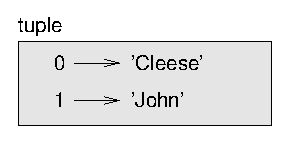
\includegraphics{figs/tuple1.eps}}
\afterfig
但是在一个更大的图中你也许希望忽略细节。例如,一个电话簿的状态图会是这样:

\beforefig
\centerline{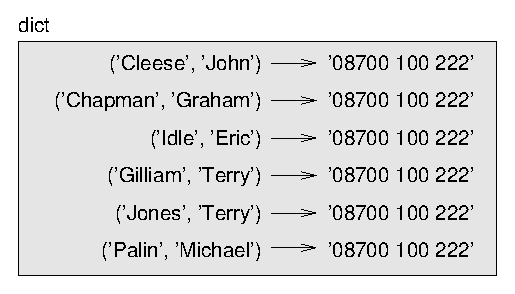
\includegraphics{figs/dict2.eps}}
\afterfig

这里元组根据Python的语法以图形速记的形式给出。

图中的电话号码是BBC的投诉电话,请不要拨打。



\section{元组比较}

\index{比较!元组}
\index{元组!比较}
\index{sort方法}
\index{方法!sort}

关系运算符使用于元组和其他序列。Python从每个序列的第一个元素开始比较。如果它们相同,则继续比较下一个元素,依次类推,直到找到有区别的元素,以后的元素将不被考虑(即使它们很大)。

\beforeverb
\begin{verbatim}
>>> (0, 1, 2) < (0, 3, 4)
True
>>> (0, 1, 2000000) < (0, 3, 4)
True
\end{verbatim}
\afterverb
%
{\tt sort}函数的工作原理类似,它根据第一个元素排序,如果第一个元素相同,则对第二个元素进行排序,依次类推。

这个特点对应{\bf DSU}模式: 

\begin{description}

\item[Decorate] 装饰序列,生成元组列表,将一个或多个排序关键字放在元素的最前面。

\item[Sort] 对元组列表排序

\item[Undecorate] 通过从已排序的序列中抽出元素来还原。

\end{description}

\label{DSU}
\index{DSU模式}
\index{模式!DSU}
\index{装饰-排序-还原模式}
\index{模式!装饰-排序-还原}

例如,假设你有列单词,你需要从最长到最短将它们排序:

\beforeverb
\begin{verbatim}
def sort_by_length(words):
    t = []
    for word in words:
       t.append((len(word), word))

    t.sort(reverse=True)

    res = []
    for length, word in t:
        res.append(word)
    return res
\end{verbatim}
\afterverb
%
第一个循环构造了一个元组列表,每个元组有单词长度和单词组成。

{\tt sort}函数首先比较第一个元素,即单词长度,仅当单词长度相同时才考虑第二个元素。关键字参数{\tt reverse=True}告诉{\tt sort}使用降序排序。

\index{关键字参数}
\index{参数!关键字}
\index{遍历}

第二个循环遍历元组列表,构建一个按长度递减排列的单词列表。

\begin{ex}
在这个例子中,长度相同的单词是按照字母顺序排序的。对于一些其他的应用,你也许需要它们是随机排序的。修改例子是长度相同的单词随机排序。提示:参考{\tt random}模块中的{\tt random}函数。


\index{random模块}
\index{模块!random}
\index{random函数}
\index{函数!random}

\end{ex}


\section{序列的序列}
\index{序列}

我主要使用元组的列表,事实上几乎本章所有的例子都还可以使用列表的列表,元组的元组和列表的元组来实现。为了避免枚举可能的组合,有时说成序列的序列更为方便。

在很多情况下,不同的序列(字符串,列表和元组)可以交换的使用。那么该如何选择,为什么这么选择呢?

\index{字符串}
\index{列表}
\index{元组}
\index{可改变}
\index{不可改变}

显而易见的是,字符串相比其他序列受到更多的限制,因为元素必须是字符。同时它们是不可改变的。如果你需要能够修改字符串中的字符(而非创建一个新的字符串),你需要使用字符的列表。

列表比元组更为常用,主要因为它们是可改变的。但有一些情况你或许会更倾向于元组:

\begin{enumerate}

\item 在某些情况下,如{\tt return}语句,语法上创建一个元组比创建一个列表更方便。在其他情况下,你也许更倾向列表。

\item 如果你要使用一个类似字典关键字的序列,你必须使用类似元组或字符串的不可改变的数据类型。

\item 如果你将序列作为函数参数,使用元组会减小潜在的因为别名而造成的意外的行为。

\end{enumerate}

由于元组是不可改变的,它们不提供类似{\tt sort}或{\tt reverse}等修改列表的方法。但是Python提供内建函数{\tt sorted}和{\tt reversed},它们读取任何序列作为参数,并返回一个新的排序后的列表。

\index{sorted函数}
\index{函数!sorted}
\index{reversed函数}
\index{函数!reversed}


\section{调试}

\index{调试}
\index{数据结构}
\index{形状错误}
\index{错误!形状}
列表、字典和元组通常被成为{\bf 数据结构}。本章中我们开始接触复合数据结构,如元组的列表、以元组作为键列表作为值的字典。复合数据结构十分有用,但它们容易造成我习惯称呼的{\bf 形状错误},即由于数据结构含有错误的类型、大小或符合而造成的错误。例如,你期望得到一个只含一个整数的列表,而我给你的是一个整数(不是一个列表),这将导致错误。

\index{structshape模块}
\index{模块!structshape}

为了帮助调试此类错误,我编写了一个叫做{\tt structshape}的模块,提供一个{\tt structshape}函数,它可以读取任何数据结构作为参数,并返回一个描述该结构的字符串。你可以在\url{thinkpython.com/code/structshape.py}下载。

下面给出一个简单列表的结果:

\beforeverb
\begin{verbatim}
>>> from structshape import structshape
>>> t = [1,2,3]
>>> print structshape(t)
list of 3 int
\end{verbatim}
\afterverb
%
更好的程序也许会输出``list of 3 int{\em s},'',但不考虑复数相对简单。下面是一个列表的列表:

\beforeverb
\begin{verbatim}
>>> t2 = [[1,2], [3,4], [5,6]]
>>> print structshape(t2)
list of 3 list of 2 int
\end{verbatim}
\afterverb
%
如果列表中的元素不是同一数据类型,{\tt structshape}按类型聚合它们:

\beforeverb
\begin{verbatim}
>>> t3 = [1, 2, 3, 4.0, '5', '6', [7], [8], 9]
>>> print structshape(t3)
list of (3 int, float, 2 str, 2 list of int, int)
\end{verbatim}
\afterverb
%
下面是一个元素的列表:

\beforeverb
\begin{verbatim}
>>> s = 'abc'
>>> lt = zip(t, s)
>>> print structshape(lt)
list of 3 tuple of (int, str)
\end{verbatim}
\afterverb
%
下面是有3项从整数到字符串映射的字典。

\beforeverb
\begin{verbatim}
>>> d = dict(lt) 
>>> print structshape(d)
dict of 3 int->str
\end{verbatim}
\afterverb
%
如果你在跟踪数据结构时遇到了问题,{\tt structshape}可以帮助你。


\section{术语}

\begin{description}

\item[元组:] 不可改变的元素的序列。
\index{元组}

\item[元组赋值:] 一个序列在右、一个元组变量在左的赋值。右边首先计算值,然后将其元素赋值给左边的变量。
\index{元组赋值}
\index{赋值!元组}

\item[聚集:] 对变长参数元组的集合操作。
\index{聚集}

\item[散布:] 将序列作为参数列表的操作。
\index{散布}

\item[DSU:] ``decorate-sort-undecorate''的简称,一个构建元组列表、排序、提取结果的模式。
\index{DSU模式}

\item[数据结构:] 相关数据的集合,通常组织为列表、字典、元组等。
\index{数据结构}

\item[形状(数据结构的):] 对数据结构类型、大小和组成的概述。
\index{形状}

\end{description}


\section{练习}

\begin{ex}
编写函数\verb"most_frequent",参数为一个字符串,以频率降序打印字符出现的次数。从不同语言的测试文本中寻找频率的不同。将你的结果和\url{wikipedia.org/wiki/Letter_frequencies}中的表格作比较。

\index{字母频率}
\index{频率!字母}

\end{ex}


\begin{ex}
\label{回文}

\index{回文集合}
\index{集合!回文}

更多关于回文的练习!

\begin{enumerate}

\item 编写函数,从文件中读取一个单词表(参考章节~\ref{单词表}),打印所有回文的单词。

下面的例子给出可能的输出结果:

\beforeverb
\begin{verbatim}
['deltas', 'desalt', 'lasted', 'salted', 'slated', 'staled']
['retainers', 'ternaries']
['generating', 'greatening']
['resmelts', 'smelters', 'termless']
\end{verbatim}
\afterverb
%
提示:你也许需要构建一个字典满足从字母的集合到这些字母可以组成的单词列表的映射。问题是你如何表示这个字母集合使得它们可以作为字典的键?

\item 修改之前的程序,使程序按照结果集合的大小从大到小输出。

\index{拼字游戏}
\index{bingo}

\item 在拼字游戏中,如果你手头的7个字母和桌面上的1个字母组成一个8个字母的单词,你实现了“bingo”。哪8个字母组成的集合有最大的概率实现“bingo”?提示:有7组。

% (7, ['angriest', 'astringe', 'ganister', 'gantries', 'granites',
% 'ingrates', 'rangiest'])

\index{置换}

\item 我们定义两个单词为“置换对”,如果你能通过交换字母顺序将一个单词转换为另一个单词\footnote{这个练习受\url{puzzlers.org}中一个例子的启发。}。例如,“converse”和“conserve”是一对“置换对”。提示:不要测试所有的单词对,也不要测试所有的交换。

你可以在\url{thinkpython.com/code/anagram_sets.py}下载一个解答。

\end{enumerate}
\end{ex}



\begin{ex}

\index{Car Talk}
\index{难题}

下面是另一个Car Talk难题\footnote{\url{www.cartalk.com/content/puzzler/transcripts/200651}。}:

\begin{quote}
如果每次你从一个单词中删除一个字母它仍是一个有效的英语单词,在英语中满足这样条件的最长的单词是什么?

删除的字母可以位于两端或者中间,但是你不能重新排列字母。每次你删除一个字母,你得到另一个英语单词。最终你得到一个只有一个字母的单词。我要知道最长的单词是什么,它有多少字母?

我要给出一个例子:Sprite。你从sprite开始删除字母,首先删除r,我们得到单词spite,接着删除e,我们得到spit,再删除s,我们得到pit,it和I。
\end{quote}

\index{可缩小的单词}
\index{单词,可缩小的}

编写程序,找出可以按这中方法缩小的所有单词,并找出最长的一个。

这个练习比以往的都更有挑战性,所以给出一些建议:

\begin{enumerate}

\item 你也许需要编写一个函数,参数为一个单词,函数找出所有删除一个字母后仍合法的单词,即原单词的“孩子”。

\index{递归定义}
\index{定义!递归}

\item 递归的看,一个单词是可缩小的,如果它所有的孩子都是可缩小的。作为基本状态,你可以认为空字符串是可以缩小的。

\item 我提供的单词表{\tt words.txt}中不包括单字母的单词。所以你需要添加“I”,“a”和空字符串。

\item 为了提高你的程序的效率,你需要记住已知的可缩小的单词。

\end{enumerate}

你可以在\url{thinkpython.com/code/reducible.py}下载我的解答。

\end{ex}
